\section{Truncations, finite conditions and the road to RH}\label{ch:rz4}

Cutting the series for $S_2$ in Theorem~\ref{rz:thm:bpy} after $n$ terms gives variables whose Mellin transforms are explicit, each a gamma factor times an exponential polynomial, with zeros that converge to the points $\rho/2$; a condition on these zeros, holding for infinitely many $n$, implies RH. We follow this route to the point where it stops. The one sided condition fails because the truncated zeros approach the critical line from a side fixed by an explicit constant $\kappa(\rho)$, and the side changes at zeros where $|S(\gamma)|$ is large, with $S(t)=\pi^{-1}\arg\zeta(\frac12+it)$ as in Appendix~\ref{app:notation}; the first such zero is $\gamma_{213}$. Symmetrising by the functional equation removes this mechanism. The resulting Conjecture S is proved above explicit heights for $n\le6$ and $n=8$ and checked numerically below them; for the other $n\le24$ and for $n=32,36$ it follows above explicit heights from torus bounds proved in ball arithmetic, and is checked numerically below them. Section~\ref{rz:sec:towards} sets the reductions of Chapter~\ref{chap:rzeta} and of this chapter against what is proved unconditionally: Weil's criterion in Thorin coordinates, Weil positivity on the Bernstein cone, the reach of finite order tests, the de Bruijn Newman flow and GGC multipliers. Sections~\ref{rz:sec:num}, \ref{rz:sec:disc} and \ref{rz:sec:open} record the numerical verification of both chapters, say what their results mean for the Thorin approach, and state open problems.

\subsection{Truncations of the Biane, Pitman and Yor lattice}\label{rz:sec:finite}

In this subsection $w$ is the complex variable of a Mellin transform and $u=w+1$; the canonical function $w(x)$ of Theorem~\ref{rz:thm:w} does not return until Section~\ref{rz:sec:towards}. The results are of three kinds. The Hurwitz reductions, the first order expansion of the truncated zeros, the formula for its constant and the single term bound for small $n$ are theorems. The argument principle counts are computations in floating point. Corollary~\ref{rz:cor:Tfalse} rests in addition on an enclosure of $\Re\kappa(\rho_{213})$ in ball arithmetic, and the results for $n=7$, $9\le n\le24$ and $n=32,36$ on bounds over a torus, proved by a branch and bound whose final boxes are enclosed in ball arithmetic.

\subsubsection{Truncated lattices and Conjecture T}

Let $e_k,e_k'$ be independent standard exponential variables, and put $\mathcal S=\sum_{k\ge1}k^{-2}(e_k+e_k')=\frac{\pi^2}2S_2$, with $S_2$ the variable of Theorem~\ref{rz:thm:bpy}, and $\mathcal S_n=\sum_{k\le n}k^{-2}(e_k+e_k')$, a GGC with finitely many Thorin atoms. Put $F(w)=\E\mathcal S^w$ and $F_n(w)=\E\mathcal S_n^w$ for $\Re w>-2$. By Theorem~\ref{rz:thm:bpy},
\[
F(w)=2\pi^{w}\,\xi(2w),
\]
so the zeros of $F$ are the points $w=\rho/2$, and RH says they lie on $\Re w=\frac14$. Each $F_n$ is explicit. Define $\alpha_k$ and $\beta_k$, which depend on $n$, by the partial fraction expansion
\[
\prod_{j\le n}\Bigl(1+\frac\lambda{j^2}\Bigr)^{-2}=\sum_{k\le n}k^{-2}\Bigl\{\alpha_k\Bigl(1+\frac\lambda{k^2}\Bigr)^{-1}+\beta_k\Bigl(1+\frac\lambda{k^2}\Bigr)^{-2}\Bigr\},
\]
so that $\beta_k=k^2\prod_{j\le n,\,j\ne k}(1-k^2/j^2)^{-2}$ and $\alpha_k=-2\beta_k\sum_{j\le n,\,j\ne k}k^2/(j^2-k^2)$; for $n=2$ they are $\beta=(\frac{16}9,\frac49)$ and $\alpha=(-\frac{32}{27},\frac{32}{27})$. The left side is the Laplace transform of $\mathcal S_n$, whose density is therefore $\sum_k(\alpha_k+\beta_kk^2x)e^{-k^2x}$, and taking moments gives, with $u=w+1$, $F_n(u-1)=\Gamma(u)Q_n(u)$, where $Q_n(u)=\sum_{k\le n}k^{-2u}(\alpha_k+\beta_ku)$. So $F_n$ is, up to $\Gamma$, an exponential polynomial with frequencies $2\log k$ and coefficients linear in $u$.

\begin{theorem}\label{rz:thm:hurwitzrh}
If for infinitely many $n$ the function $F_n$ has no zeros in the half plane $\Re w>\frac14$, then the Riemann Hypothesis holds.
\end{theorem}

\begin{proof}
For $\Re w>-2$ the variables $\mathcal S_n^w$ are dominated by an integrable variable, since $\mathcal S_n\ge e_1+e_1'$ and $\mathcal S_n\le\mathcal S$, so $F_n\to F$ locally uniformly on $\Re w>-2$. If $F$ had a zero $w_0$ with $\Re w_0>\frac14$, Hurwitz's theorem would give zeros of $F_n$ near $w_0$ for all large $n$. Hence every zero $\rho/2$ of $F$ has $\Re\rho\le\frac12$, and the symmetry $\rho\mapsto1-\rho$ gives $\Re\rho=\frac12$.
\end{proof}

Asking for the hypothesis at every $n$ gives the simplest condition of this kind.

\medskip
\noindent\textsc{Conjecture T.} For every $n\ge1$, $F_n(w)=\E\bigl[\bigl(\sum_{k\le n}k^{-2}(e_k+e_k')\bigr)^w\bigr]$ has no zeros with $\Re w>\frac14$.
\medskip

By Theorem~\ref{rz:thm:hurwitzrh}, Conjecture T implies RH. It is a stability statement, of Hermite Biehler or Lee and Yang type \cite{LeeYang}, for a sequence of explicit exponential polynomials. It is false (Corollary~\ref{rz:cor:Tfalse}, whose proof uses an enclosure of $\Re\kappa(\rho_{213})$ in ball arithmetic), and we state it because the mechanism of its failure also defeats, for large $n$, the Hermite Biehler inequality on which the bounds of Theorems~\ref{rz:thm:Yn} and \ref{rz:thm:torus} for the symmetrised truncations rest.

At small $n$ the evidence supports it: Table~\ref{rz:tab:Trect} finds no zero of $Q_n$ with $\Re u>\frac54$ in any rectangle searched. The zeros are counted by the argument principle, with $800$ to $4000$ sample points per side and a working precision of $40$ to $340$ decimal digits to control the cancellation among the partial fraction coefficients, and located by Newton's method from a grid; the counts and the zeros found agree.

\begin{table}[htbp]
\centering
\small
\begin{tabular}{lll}
\toprule
$n$ & region, in $u=w+1$ & zeros with $\Re u>\frac54$\\
\midrule
$2,3,4,5,6,8,12,16,24,32$ & $\frac54<\Re u<6$, $0.3<\Im u<40$ & none\\
$8,16,32$ & $\frac54<\Re u<6$, $40<\Im u<100$ & none\\
$48,64$ & $\frac54<\Re u<6$, $0.3<\Im u<30$ & none\\
$16,32,64$ & $6<\Re u<40$, $0.3<\Im u<40$ & none\\
\bottomrule
\end{tabular}
\caption{Argument principle counts for Conjecture T: rectangles searched and zeros of $Q_n$ found with $\Re u>\frac54$.}
\label{rz:tab:Trect}
\end{table}

Rectangles to the left of the line contain the expected zeros: $8$, $12$, $12$, $15$, $15$, $17$, $18$, $19$, $21$, $21$ zeros with $-6<\Re u<\frac54$ and $\Im u<40$ for the ten values of $n$ in the first row. For $n=2$ the eight zeros found lie on $\Re u=-1$ exactly. On the real axis $F_n$ is positive, and for fixed $n$ and large $|\Im u|$ the zeros move far to the left, because the extreme coefficients $\beta_1$ and $\beta_n$ differ by a factor of order $16^n$, up to a power of $n$. The intermediate heights are therefore where Conjecture T is at risk, and they are the heights that Table~\ref{rz:tab:Trect} searches; the failure found in Corollary~\ref{rz:cor:Tfalse} lies above them (Remark~\ref{rz:rem:firstordergap}). An experiment shows that the absence of such zeros at small $n$ is not a consequence of the GGC structure alone: replacing the weights $k^{-2}$ by $k^{-2}(1+\eta_k)$, with independent $\eta_k$ uniform on $[-0.15,0.15]$, one of two draws at $n=16$ gives a zero with $\Re u>\frac54$. The property depends on the exact quadratic lattice.

\subsubsection{How the truncated zeros reach the line, and why Conjecture T fails}

Near a simple zero $\rho$ of $\xi$, the zeros of $F_n$ converge to $\rho/2$ at rate $1/n$, with an explicit constant.

\begin{proposition}\label{rz:prop:firstorder}
Let $\rho$ be a simple zero of $\xi$ and put
\[
\kappa(\rho)=\frac{\rho\,\xi(\rho-2)}{2\pi\,\xi'(\rho)}=\frac{\rho\,\xi(3-\rho)}{2\pi\,\xi'(\rho)} .
\]
There is a constant $C$ such that for all large $n$, $F_n$ has exactly one zero $w_n(\rho)$ in the disc $|w-\frac\rho2-\frac{\kappa(\rho)}n|<C/n^2$; thus $w_n(\rho)=\frac\rho2+\frac{\kappa(\rho)}n+O(n^{-2})$.
\end{proposition}

\begin{proof}
Write $\mathcal S=\mathcal S_n+\mathcal T_n$ with $\mathcal T_n=\sum_{k>n}k^{-2}(e_k+e_k')$, independent of $\mathcal S_n$, so that $\E\mathcal T_n=2\sum_{k>n}k^{-2}=\frac2n+O(n^{-2})$ and $\E\mathcal T_n^2=O(n^{-2})$. For $a>0$, $b\ge0$ and $0<\Re w<2$, Taylor's formula with integral remainder and $|(a+tb)^{w-2}|=(a+tb)^{\Re w-2}\le a^{\Re w-2}$ give
\begin{gather*}
\bigl|(a+b)^w-a^w-wb\,a^{w-1}\bigr|\le\tfrac12|w(w-1)|\,b^2a^{\Re w-2},\\
\bigl|(a+b)^{w-1}-a^{w-1}\bigr|\le|w-1|\,b\,a^{\Re w-2}.
\end{gather*}
Since $\mathcal S_n\ge e_1+e_1'$, a $\Gamma(2)$ variable, $\E\mathcal S_n^{\Re w-2}\le\Gamma(\Re w)$. Taking expectations with $a=\mathcal S_n$ and $b=\mathcal T_n$, and using independence,
\[
F(w)=F_n(w)+w\,\E\mathcal T_n\,F_n(w-1)+O(n^{-2}),\qquad F_n(w-1)=F(w-1)+O(n^{-1}),
\]
uniformly on compact subsets of $0<\Re w<2$. Hence $F_n(w)=F(w)-\frac2nwF(w-1)+O(n^{-2})$ uniformly there. Put $w_0=\rho/2$, so $0<\Re w_0<\frac12$, and recall $F(w_0)=0$ and $F'(w_0)=4\pi^{w_0}\xi'(\rho)\ne0$. For $|w-w_0|=O(1/n)$, Taylor expansion of $F$ and of $wF(w-1)$ about $w_0$ gives
\[
F_n(w)=F'(w_0)\Bigl(w-w_0-\frac{\kappa(\rho)}n\Bigr)+O(n^{-2}),\qquad\frac{\kappa(\rho)}n=\frac2n\,\frac{w_0F(w_0-1)}{F'(w_0)},
\]
and $F(w_0-1)=2\pi^{w_0-1}\xi(\rho-2)$ turns the second identity into the stated $\kappa$. On the circle $|w-w_0-\kappa/n|=C/n^2$ the linear term has modulus $|F'(w_0)|C/n^2$, which exceeds the $O(n^{-2})$ error once $C$ is larger than its constant divided by $|F'(w_0)|$. Rouch\'e's theorem gives exactly one zero inside for all large $n$. The second form of $\kappa$ follows from $\xi(s)=\xi(1-s)$.
\end{proof}

Each simple zero $\rho$ of $\xi$ thus has a companion zero of the truncation at distance of order $1/n$, displaced in the direction $\kappa(\rho)$. If $\Re\kappa(\rho)>0$ the companion lies to the right of the critical line for all large $n$. This happens at zeros where $|S(\gamma)|$ is large, the first being $\gamma_{213}$ (Theorem~\ref{rz:thm:kappaexact} and the computation after it), and it is why Conjecture T fails.

For each of the first $100$ zeros $\kappa(\rho)$ has negative real part, starting with $\kappa(\rho_1)=-4.762-1.944i$, $\kappa(\rho_2)=-8.673-0.627i$, $\kappa(\rho_3)=-10.149-3.872i$ and $\kappa(\rho_4)=-15.165+3.705i$. So these truncated zeros approach the critical line from the left, at distance about $-\Re\kappa(\rho)/n$, which grows with the height: $-\Re\kappa(\rho)/\gamma^2$ lies between $0.011$ and $0.024$ for the first ten zeros, with $0.024$ at $\gamma_1$ and $0.013$ at $\gamma_{10}$. Figure~\ref{rz:fig:traj} and Table~\ref{rz:tab:traj} show the approach for the first four zeros, computed by locating the zeros of $F_n$ directly at each $n$ rather than from the expansion. The convergence of $n(\frac54-\Re u)$ to $-\Re\kappa(\rho_j)$, in the right panel of the figure and the last row of the table, is an independent check on Proposition~\ref{rz:prop:firstorder} at low height.

\begin{figure}[htbp]
\centering
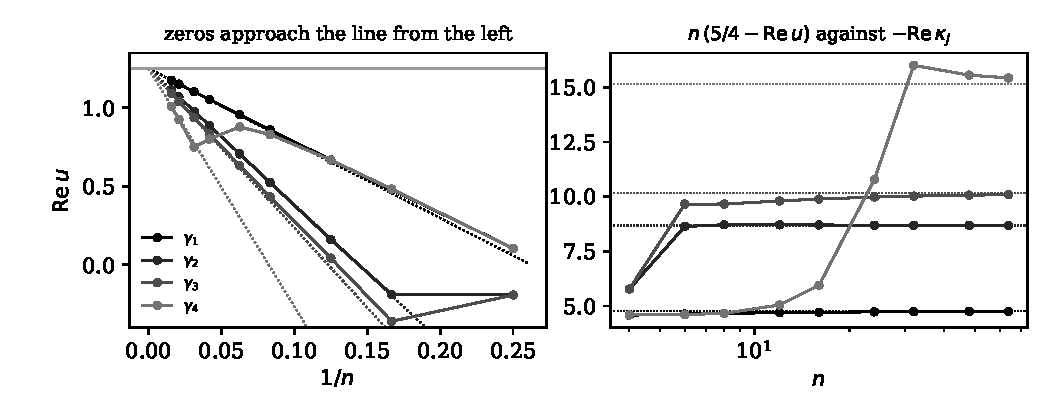
\includegraphics[width=0.95\textwidth]{rzfig/fig_traj.pdf}
\caption{Left: real parts of the zeros of $F_n$ near $\rho_j/2$, in the variable $u=w+1$, against $1/n$ for $n=4$ to $64$, with the first order lines $\frac54+\Re\kappa(\rho_j)/n$ (dotted). The zeros approach $\Re u=\frac54$, the image of the critical line, from the left. Right: $n(\frac54-\Re u)$ against $n$, converging to $-\Re\kappa(\rho_j)$.}
\label{rz:fig:traj}
\end{figure}

\begin{table}[htbp]
\centering
\footnotesize
\setlength{\tabcolsep}{4pt}
\begin{tabular}{rcccc}
\toprule
$n$ & near $\rho_1/2$ & near $\rho_2/2$ & near $\rho_3/2$ & near $\rho_4/2$\\
\midrule
$8$ & $0.6678+6.8583i$ & $0.1610+10.6538i$ & $0.0426+11.9969i$ & $0.6676+15.7727i$\\
$16$ & $0.9558+6.9550i$ & $0.7062+10.5197i$ & $0.6321+12.2722i$ & $0.8787+15.7928i$\\
$32$ & $1.1020+7.0090i$ & $0.9785+10.5029i$ & $0.9368+12.3881i$ & $0.7498+15.4606i$\\
$64$ & $1.1758+7.0376i$ & $1.1144+10.5040i$ & $1.0924+12.4460i$ & $1.0089+15.2948i$\\
limit & $1.25+7.0674i$ & $1.25+10.5110i$ & $1.25+12.5054i$ & $1.25+15.2124i$\\
$n(\frac54-\Re u)$ at $64$ & $4.75$ & $8.68$ & $10.09$ & $15.43$\\
\bottomrule
\end{tabular}
\caption{Zeros of $F_n$ near $\rho_j/2$, in the variable $u=w+1$. The row ``limit'' is $\rho_j/2+1$; the last row, $n(\frac54-\Re u)$ at $n=64$, is to be compared with $-\Re\kappa(\rho_j)=4.762$, $8.673$, $10.149$, $15.165$.}
\label{rz:tab:traj}
\end{table}

The direction from which a truncated zero reaches the line is not always the same, and the sign of $\Re\kappa(\rho)$ can be read off from Hardy's function.

\begin{theorem}\label{rz:thm:kappaexact}
Let $\rho=\frac12+i\gamma$ be a simple zero on the critical line, let $\theta$ be the Riemann Siegel theta function and $Z(t)=e^{i\theta(t)}\zeta(\frac12+it)$ Hardy's function, and put $a(\gamma)=e^{i\theta(\gamma)}\zeta(\frac52+i\gamma)$. Then
\begin{align*}
\Re\kappa(\rho)&=\frac{(\gamma^2-\frac{15}4)\Im a(\gamma)-4\gamma\Re a(\gamma)}{4\pi^2Z'(\gamma)},\\
\Im\kappa(\rho)&=\frac{4\gamma\Im a(\gamma)+(\gamma^2-\frac{15}4)\Re a(\gamma)}{4\pi^2Z'(\gamma)} .
\end{align*}
\end{theorem}

\begin{proof}
On the line $\xi(\frac12+it)=\Xi(t)$ is real, so $\xi'(\rho)=-i\,\Xi'(\gamma)$, and $\Xi(t)=-\frac12(t^2+\frac14)\pi^{-1/4}|\Gamma(\frac14+\frac{it}2)|Z(t)$ gives $\Xi'(\gamma)=-\frac12(\gamma^2+\frac14)\pi^{-1/4}|\Gamma(\frac14+\frac{i\gamma}2)|Z'(\gamma)$ at a zero. Since $\xi(3-\rho)=\xi(\frac52-i\gamma)$ and $\xi$ is real on the real axis, $\xi(3-\rho)=\overline{\xi(\frac52+i\gamma)}$, and $\Gamma(\frac54+\frac{i\gamma}2)=(\frac14+\frac{i\gamma}2)\Gamma(\frac14+\frac{i\gamma}2)$ with $\pi^{-i\gamma/2}\Gamma(\frac14+\frac{i\gamma}2)=|\Gamma(\frac14+\frac{i\gamma}2)|e^{i\theta(\gamma)}$. Substituting, the moduli of $\Gamma$ cancel, $(\frac12+i\gamma)(\frac14-\frac{i\gamma}2)=\frac12(\gamma^2+\frac14)$ cancels the remaining factor, and $\kappa=-i(\frac52-i\gamma)(\frac32-i\gamma)\overline{a(\gamma)}/(4\pi^2Z'(\gamma))$, whose real and imaginary parts are as stated.
\end{proof}

For large $\gamma$ the term $(\gamma^2-\frac{15}4)\Im a(\gamma)$ decides the sign of $\Re\kappa(\rho)$. Since $|\zeta(\frac52+i\gamma)-1|\le\zeta(\frac52)-1<0.35$, $a(\gamma)$ is a positive multiple of $e^{i\theta(\gamma)}$ up to a phase below $0.35$ in modulus, and up to that phase the sign of $\Re\kappa(\rho)$ is the sign of $\sin\theta(\gamma)/Z'(\gamma)$. Let $S_{\rm mid}$ be the midpoint of the jump of $S$ at the $n$th zero $\gamma_n$. Then $\theta(\gamma_n)=\pi(n-\frac32-S_{\rm mid})$ and the sign of $Z'(\gamma_n)$ is $(-1)^{n+1}$, so the sign of $\sin\theta(\gamma_n)/Z'(\gamma_n)$ is that of $-\cos(\pi S_{\rm mid})$: negative when $|S_{\rm mid}|<\frac12$, that is when the zero lies within half a spacing of its expected position, and positive when $\frac12<|S_{\rm mid}|<\frac32$. The phase of $\zeta(\frac52+i\gamma)$ moves the threshold $\frac12$ by at most about $0.11$ either way. For the first $460$ zeros the sign of $\Re\kappa$ agrees with the sign of $\Im a(\gamma)/Z'(\gamma)$ in every case, and $\Re\kappa>0$ occurs three times, at
\[
\gamma_{213}=415.4552,\quad\gamma_{289}=527.9036,\quad\gamma_{379}=650.6687,
\]
with $\kappa=233.96-2298.91i$, $604.16+3074.08i$, $1164.60-4296.91i$.

At these three zeros the jump of $S$ runs from $0.098$ to $1.098$, from $-1.145$ to $-0.145$ and from $0.164$ to $1.164$; the midpoints of the jumps are $0.598$, $-0.645$ and $0.664$. Seven of the first $460$ zeros have $S(\gamma^-)<-1$: besides $\gamma_{289}$ these are $\gamma_{127}$, $\gamma_{196}$, $\gamma_{233}$, $\gamma_{368}$, $\gamma_{380}$ and $\gamma_{401}$, with midpoints $-0.506$, $-0.505$, $-0.537$, $-0.556$, $-0.538$ and $-0.514$, and $\Re\kappa$ is negative at every one of them. Three further zeros have midpoints above $\frac12$ and $\Re\kappa<0$: $\gamma_{136}$, $\gamma_{256}$ and $\gamma_{399}$, at $0.507$, $0.510$ and $0.539$. The largest $|S_{\rm mid}|$ with $\Re\kappa<0$ is $0.556$, at $\gamma_{368}$, and the smallest with $\Re\kappa>0$ is $0.598$, at $\gamma_{213}$, so the threshold on the midpoint lies between about $0.56$ and $0.60$, inside the range $\frac12\pm0.11$ allowed by the phase of $\zeta(\frac52+i\gamma)$.

\begin{corollary}\label{rz:cor:Tfalse}
Conjecture T is false: for all sufficiently large $n$, $F_n$ has a zero with $\Re w>\frac14$ near $\rho_{213}/2$.
\end{corollary}

\begin{proof}
The first $1.5\times10^9$ zeros, $\rho_{213}$ among them, lie on the critical line and are simple \cite{LRW86}, and ball arithmetic applied to the formula of Theorem~\ref{rz:thm:kappaexact} gives $233.95<\Re\kappa(\rho_{213})<233.96$ (Section~\ref{rz:sec:num}). By Proposition~\ref{rz:prop:firstorder}, for all large $n$ the function $F_n$ has a zero $w_n$ with $|w_n-\frac{\rho_{213}}2-\frac{\kappa(\rho_{213})}n|<C/n^2$, so $\Re w_n>\frac14+\frac{233.95}n-\frac C{n^2}>\frac14$ once $n>C/233.95$.
\end{proof}

In particular the hypothesis of Theorem~\ref{rz:thm:hurwitzrh} fails for every large $n$.

\begin{remark}\label{rz:rem:firstordergap}
The constants in Proposition~\ref{rz:prop:firstorder} depend on $\rho$, and the first order regime requires $n$ large compared with $|\kappa(\rho)|$. For the zero $\rho_{213}$ of Corollary~\ref{rz:cor:Tfalse}, $|\kappa(\rho_{213})|=2311$, so the phenomenon begins at $n$ of order $10^3$ or beyond, larger than every $n$ computed in this section. Table~\ref{rz:tab:Trect} accordingly reports no zero with $\Re u>\frac54$, and cannot detect this one, since its rectangles reach $\Im u=100$ while the predicted failure sits at $\Im u=207.7$.
\end{remark}

The failure is intrinsic to the method, not to the particular lattice. Any truncation whose first order error is a multiple of $F(w-1)$ produces the displacement $\kappa(\rho)/n$, and the phase of $\kappa(\rho)$ is governed by $S(\gamma)$. By Selberg's central limit theorem \cite{Selberg46} $S$ takes values beyond $\pm\frac12$ for a positive proportion of heights, so one expects a positive proportion of zeros to be approached from the right. One sided Hurwitz arguments therefore cannot succeed for truncations of this kind; what is needed is a scheme in which symmetry keeps the zeros on the line.

\subsubsection{Symmetrised truncations and Conjecture S}

The functional equation supplies that symmetry. Put
\[
K_n(w)=\pi^{-w}F_n(w)+\pi^{w-\frac12}F_n(\tfrac12-w),\qquad Z_n(y)=K_n(\tfrac14+iy).
\]

\begin{proposition}\label{rz:prop:symtrunc}
$K_n(\frac12-w)=K_n(w)$, $K_n(\bar w)=\overline{K_n(w)}$, so $Z_n$ is real for real $y$ and the zeros of $K_n$ off the line $\Re w=\frac14$ come in quadruples. As $n\to\infty$, $K_n\to4\,\xi(2w)$ locally uniformly on $-\frac74<\Re w<\frac94$. Every simple zero $\frac14+i\frac\gamma2$ of $\xi(2w)$ on the line is, for all large $n$, the limit of a zero of $K_n$ lying exactly on the line.
\end{proposition}

\begin{proof}
The symmetries are immediate from the definition and the reality of $F_n$ on the real axis. The limit follows from $F_n\to F=2\pi^w\xi(2w)$ and $\xi(1-2w)=\xi(2w)$; since $F_n\to F$ on $\Re w>-2$, the convergence holds on $-2<\Re w<\frac52$, which contains the strip of the statement. Near a simple zero $y_0$ of the real function $4\xi(\frac12+2iy)$, $Z_n$ converges uniformly and so changes sign near $y_0$; by Hurwitz, $K_n$ has exactly one zero near $\frac14+iy_0$, which must be the real zero of $Z_n$, since an off line zero would bring its mirror image $\frac12-\bar w$ with it.
\end{proof}

So for symmetrised truncations the local mechanism that broke Conjecture T is absent: a simple zero on the line cannot leave it under a small symmetric perturbation; it can leave only after colliding with another zero. The Hurwitz argument now gives the following.

\begin{theorem}\label{rz:thm:symhurwitz}
If for infinitely many $n$ all zeros of $K_n$ in the strip $0<\Re w<\frac12$ lie on the line $\Re w=\frac14$, then RH holds.
\end{theorem}

\begin{proof}
A zero $\rho/2$ of $\xi(2w)$ off the line lies in the strip $0<\Re w<\frac12$, since $0<\Re\rho<1$, and by Hurwitz it is the limit of zeros of $K_n$ in the strip, which would be off the line for large $n$.
\end{proof}

\medskip
\noindent\textsc{Conjecture S.} For every $n\ge1$, all zeros of $K_n$ in $0<\Re w<\frac12$ lie on $\Re w=\frac14$.
\medskip

The symmetrised zeros move along the line. The first order argument of Proposition~\ref{rz:prop:firstorder}, applied to $K_n=2\Re[\pi^{-w}F_n(w)]$ on the line, gives
\[
w_n^{\mathrm{sym}}(\rho)=\frac\rho2+\frac{i\,\Im\kappa(\rho)}n+O(n^{-2}):
\]
the symmetrisation removes the real part of the displacement, which is the part that broke Conjecture T, and keeps the imaginary part. Numerically the first two symmetrised zeros are at $\Im w=7.0328,7.0072,7.0231,7.0413$ and $10.5490,10.5392,10.5161,10.5085$ for $n=8,16,32,64$, against the first order values $7.0370$ and $10.5012$ at $n=64$.

\begin{table}[htbp]
\centering
\small
\begin{tabular}{llll}
\toprule
$n$ & window in $\Im w$ & \begin{tabular}[b]{@{}l@{}}zeros in $-4<\Re w<4.5$:\\ total, on the line\end{tabular} & zeros of $\xi$\\
\midrule
$1$ & $(0.5,40)$, $(40,70)$ & $23,21$; $27,27$ & $21$; $27$\\
$2$ & $(0.5,40)$, $(40,70)$ & $23,21$; $27,27$ & $21$; $27$\\
$3$ & $(0.5,40)$, $(40,70)$ & $23,21$; $27,27$ & $21$; $27$\\
$4,5,6,8,16$ & $(0.5,40)$, $(40,70)$ & $21,21$; $27,27$ & $21$; $27$\\
$32$ & $(0.5,40)$ & $21,21$ & $21$\\
$8$ & $(70,140)$, $(195,215)$ & $78,78$; $27,27$ & $78$; $26$\\
\bottomrule
\end{tabular}
\caption{Zeros of the symmetrised truncations $K_n$ in $-4<\Re w<4.5$: total found, how many lie on the line, and the number of zeros of $\xi$ in the doubled window for comparison. In the window $195<\Im w<215$ the count for $K_8$ exceeds that for $\xi$ by one; see the text.}
\label{rz:tab:symwin}
\end{table}

Table~\ref{rz:tab:symwin} counts the zeros of $K_n$ in windows of height. For $n=1$ the one off line quadruple lies at $\Re w=-2.001,2.501$, $\Im w=\pm2.471$, and for $n=2$ at $\Re w=-2.949,3.449$, $\Im w=\pm3.261$, far from the critical strip and near the region where the truncations stop resembling $\xi$; for $n=3$ it is similar. These quadruples have $|\Re w-\frac14|>2$, so they lie outside the strip $0<\Re w<\frac12$ of Theorem~\ref{rz:thm:symhurwitz} and do not bear on Conjecture S. For $n\ge4$ every zero found lies on the line. In the first three windows the counts on the line equal the numbers of zeros of $\xi$ in the doubled range, as the last column records; the totals for $n=1,2,3$ are larger because of the off line quadruple. The positions converge to $\gamma/2$: for $n=16$ the first four zeros, located on a grid of step $0.01$, are at $7.005$, $10.535$, $12.465$, $15.295$ against $7.067$, $10.511$, $12.505$, $15.212$; located more precisely, the first two are at $7.0072$ and $10.5392$.

The window $195<\Im w<215$ matters because it contains $\gamma_{213}/2=207.73$, where the unsymmetrised truncations are forced off the line. There the count for $K_8$ exceeds that for $\xi$ by one: the zeros of $\xi$ with $390<\gamma<430$ are $\gamma_{196}$ to $\gamma_{221}$, twenty six of them, the nearest excluded ordinates being $\gamma_{195}=388.85$ and $\gamma_{222}=430.33$. The difference is not a contradiction: at this height and $n=8$ the first order displacement along the line, $\Im\kappa(\rho)/n$, is of order $300$ for $\rho_{213}$, so $K_8$ is far from its limit and its zeros need not correspond one to one with those of $\xi$. What matters for Conjecture S is that every zero found in the window lies on the line.

The symmetrised truncations are the lattice analogue of the approximations $\zeta_N(s)=\sum_{m\le N}m^{-s}+\chi(s)\sum_{m\le N}m^{s-1}$ derived from the approximate functional equation, with $\chi$ the factor in $\zeta(s)=\chi(s)\zeta(1-s)$. Spira \cite[Section 6]{Spira67} and Gonek and Montgomery \cite{GonekMontgomery13} studied their zeros, and Gonek and Montgomery proved that for $N\le T^{o(1)}$ almost all zeros of $\zeta_N$ with ordinates in $[0,T]$ lie on the critical line and are simple. For $K_n$ the off line zeros found disappear from $n=4$ on, in every window examined. A proof of Conjecture S for infinitely many $n$ would require controlling the zeros of $Z_n$ uniformly in height, including the range of heights comparable with $n$, where $K_n$ is neither close to $4\xi(2w)$ nor dominated by a single exponential term; this is the same difficulty as for $\zeta_N$, now for an exponential polynomial with gamma lattice coefficients.

\subsubsection{A single term bound for small \texorpdfstring{$n$}{n}}

For small $n$, Conjecture S reduces to a finite computation, because at large heights the gamma factor makes $\log|A_n|$ increase across the strip. Here $A_n(w)=\pi^{-w}F_n(w)$, so that $K_n(w)=A_n(w)+A_n^*(w)$ with $A_n^*(w)=A_n(\frac12-w)$ and $|A_n^*(\sigma+iy)|=|A_n(\frac12-\sigma+iy)|$. If $\sigma\mapsto\log|A_n(\sigma+iy)|$ is increasing on $(0,\frac12)$, then $|A_n|>|A_n^*|$ for $\frac14<\sigma<\frac12$, and $K_n$ has no zeros there at height $y$; by symmetry none to the left of the line either. The derivative is $\Re\frac{A_n'}{A_n}=-\log\pi+\Re\psi(w+1)+\Re\frac{Q_n'}{Q_n}(w+1)$, and for large $y$ the digamma term dominates.

\begin{theorem}\label{rz:thm:Yn}
Let $Q_n(u)=\sum_kk^{-2u}(\alpha_k+\beta_ku)$ as above and, for $y>|\alpha_1|/|\beta_1|$, let $\delta_n(y)=\sum_{k\ge2}k^{-2}\frac{|\beta_k|y+|\alpha_k|}{|\beta_1|y-|\alpha_1|}$ and
\[
\delta_n'(y)=\sum_{k\ge2}k^{-2}\frac{2\log k\,(|\beta_k|y+|\alpha_k|)+|\beta_k|}{|\beta_1|y-|\alpha_1|}+\delta_n(y)\,\frac{|\beta_1|}{|\beta_1|y-|\alpha_1|},
\]
which bounds a derivative in the proof and is not the derivative of $\delta_n$. If $\delta_n(y)<1$ and
\[
\log\frac y\pi-\frac1y-\frac{|\beta_1|}{|\beta_1|y-|\alpha_1|}-\frac{\delta_n'(y)}{1-\delta_n(y)}>0,
\]
then $K_n$ has no zeros off the line in $0<\Re w<\frac12$ at any height $\ge y$. The condition holds for all $y\ge Y_n$, with $Y_1=4.81$, $Y_2=5.85$, $Y_3=7.11$, $Y_4=9.08$, $Y_5=12.8$, $Y_6=20.8$, $Y_8=104.1$ and $Y_{10}=21232$.
\end{theorem}

\begin{proof}
$|\psi(z)-\log z|\le1/|z|$ for $\Re z\ge1$, so $\Re\psi(w+1)\ge\log y-\frac1y$ at height $y$. Write $Q_n(u)=(\alpha_1+\beta_1u)(1+\delta(u))$. On $1\le\Re u\le\frac32$, $|u|\ge y$, we have $|k^{-2u}|\le k^{-2}$, so $|\delta(u)|\le\delta_n(y)$, and differentiating the quotient $\delta(u)$ term by term gives $|\delta'(u)|\le\delta_n'(y)$; both bounds decrease in $y$. Then $\Re\frac{Q_n'}{Q_n}\ge-\frac{|\beta_1|}{|\alpha_1+\beta_1u|}-\frac{|\delta'|}{1-|\delta|}$, and the condition makes $\Re(A_n'/A_n)>0$ on the strip at every height $\ge y$. The values of $Y_n$ come from evaluating these bounds with the exact coefficients.
\end{proof}

\begin{corollary}\label{rz:cor:Ssmall}
Conjecture S holds for $n=1,2,3,4,5,6,8$ above the heights $Y_n$ of Theorem~\ref{rz:thm:Yn}, and is verified numerically below them, by a floating point argument principle count and not by an enclosure.
\end{corollary}

\begin{proof}
Above $Y_n$ this is Theorem~\ref{rz:thm:Yn}. Below it, the argument principle counts cover the strip $0<\Re w<\frac12$ for $0<\Im w<6,7,8$ when $n=1,2,3$, and the windows of Table~\ref{rz:tab:symwin} cover $0<\Im w<70$ for $4\le n\le6$ and $0<\Im w<140$ for $n=8$, with $0<\Im w<0.6$ checked separately and $K_n>0$ on the real segment; in each case the total count in the strip equals the number of sign changes of $Z_n$ on the line. The counts use $40$ or more digits and fine sampling.
\end{proof}

The single term bound of Theorem~\ref{rz:thm:Yn} deteriorates quickly: the lattice coefficients $|\beta_k/\beta_1|$ grow with $n$ (they are $1.96$, $1.31$, $0.40$ for $k=2,3,4$ at $n=8$), $Y_{10}=21232$, and for $n\ge12$ the bound fails because $\delta_n>1$. A torus version removes most of this loss.

\subsubsection{Torus bounds and where they stop}

Write $u=x+iy$ and $Q_n(u)=u\,P_n(u)+R_n(u)$ with the Dirichlet polynomials $P_n(u)=\sum_{k\le n}\beta_kk^{-2u}$ and $R_n(u)=\sum_{k\le n}\alpha_kk^{-2u}$. At height $y$ the values of $P_n$ depend on $y$ only through the prime phases $(p^{-2iy})_{p\le n}$, which lie on the torus $\mathbb T^{\pi(n)}$. Replacing them by independent phases $\omega=(\omega_p)_{p\le n}\in\mathbb T^{\pi(n)}$ gives the torus function
\[
P_n(x,\omega)=\sum_{k\le n}\beta_kk^{-2x}\exp\Bigl(-i\sum_{p\le n}v_p(k)\,\omega_p\Bigr),
\]
where $v_p(k)$ is the exponent of $p$ in $k$, and in the same way the torus function $P_n'(x,\omega)$ of $P_n'(u)=-\sum_k2\log k\,\beta_kk^{-2u}$. Their extremes over the torus bound the values at every height. Put $r(x)=\sum_k|\alpha_k|k^{-2x}$ and $r'(x)=\sum_k2\log k\,|\alpha_k|k^{-2x}$.

\begin{theorem}\label{rz:thm:torus}
Let $m_n=\min|P_n(x,\omega)|$, $M_n=\max\{-\Re(P_n'/P_n)(x,\omega)\}$ and $\ell_n=\max|P_n'/P_n|(x,\omega)$, over $\omega\in\mathbb T^{\pi(n)}$ and the band $1.2\le x\le1.3$, and let
\[
B_n(y)=\max_{0.3\le\sigma\le\frac12,\ \omega}\frac{\splitfrac{\log\bigl(|P_n(\frac32-\sigma,\omega)|+r(\frac32-\sigma)/y\bigr)}{-\log\bigl(|P_n(1+\sigma,\omega)|-r(1+\sigma)/y\bigr)}}{2\sigma-\frac12}.
\]
If $m_n>r(1.2)/y$,
\[
\log\frac y\pi-\frac2y-M_n-\frac{\ell_nr(1.2)+r'(1.2)+r(1.2)/y}{y\,(m_n-r(1.2)/y)}>0\quad\text{and}\quad\log\frac y\pi-\frac1y>B_n(y),
\]
then $K_n$ has no zeros off the line in $0<\Re w<\frac12$ at height $y$, and the same holds at every larger height.
\end{theorem}

\begin{proof}
For $\frac14<\sigma\le0.3$ both $\sigma$ and $\frac12-\sigma$ lie in $[0.2,0.3]$, and the first condition makes $\Re(A_n'/A_n)>0$ there: $\Re\psi(w+1)\ge\log y-\frac1y$, $\Re\frac1u>0$, and $\frac{Q_n'}{Q_n}=\frac1u+\frac{P_n'+R_n'/u-R_n/u^2}{P_n+R_n/u}$ differs from $\frac1u+\frac{P_n'}{P_n}$ by at most the stated correction. So $\log|A_n|$ increases on $[\frac12-\sigma,\sigma]$ and $|A_n|>|A_n^*|$. For $0.3\le\sigma\le\frac12$ compare directly: $\log|\Gamma(1+\sigma+iy)|-\log|\Gamma(\frac32-\sigma+iy)|\ge(2\sigma-\frac12)(\log y-\frac1y)$ by integrating $\Re\psi$, $|1+\sigma+iy|>|\frac32-\sigma+iy|$, and $|P_n+R_n/u|$ is bounded below on the right by $|P_n|-r/y$ and above on the left by $|P_n|+r/y$; the second condition then gives $|A_n(\sigma+iy)|>|A_n(\frac12-\sigma+iy)|$. Both conditions improve as $y$ increases.
\end{proof}

Table~\ref{rz:tab:torus} lists bounds for the torus extremes, proved by a branch and bound over the band and the torus (Remark~\ref{rz:rem:torus}), and the smallest integer heights at which the first condition holds with these bounds. The second condition holds there too: the same branch and bound proves it at a height below each threshold, and it improves as $y$ increases. For $n=7$ and $9\le n\le15$ we use a single band variant: if $m_n>r(1)/y$ and the first condition of Theorem~\ref{rz:thm:torus} holds with $m_n$, $M_n$, $\ell_n$ the extremes over the band $1\le x\le\frac32$ and with $r(1)$, $r'(1)$ in place of $r(1.2)$, $r'(1.2)$, then $\Re(A_n'/A_n)>0$ on $0<\Re w<\frac12$ at height $y$, so $\log|A_n|$ increases across the strip and $K_n$ has no zeros off the line there; the condition improves as $y$ increases. The proof is the first part of the proof of Theorem~\ref{rz:thm:torus} with the band widened, since $r$ and $r'$ decrease in $x$ and $\Re\psi(w+1)\ge\log y-\frac1y$ on the whole strip. Table~\ref{rz:tab:torus1} gives the bounds and thresholds of this variant.

\begin{table}[htbp]
\centering
\small
\setlength{\tabcolsep}{3pt}
\begin{tabular}{rccccccccccc}
\toprule
$n$ & $16$ & $17$ & $18$ & $19$ & $20$ & $21$ & $22$ & $23$ & $24$ & $32$ & $36$\\
\midrule
$m_n\ge$ & $1.062$ & $1.003$ & $0.947$ & $0.895$ & $0.846$ & $0.800$ & $0.757$ & $0.716$ & $0.677$ & $0.361$ & $0.203$\\
$M_n\le$ & $0.862$ & $0.895$ & $0.926$ & $0.956$ & $0.985$ & $1.012$ & $1.039$ & $1.064$ & $1.089$ & $1.259$ & $1.331$\\
$\ell_n\le$ & $3.600$ & $3.948$ & $4.310$ & $4.689$ & $5.086$ & $5.504$ & $5.954$ & $6.473$ & $7.075$ & $17.203$ & $33.568$\\
$r(1.2)\le$ & $7.522$ & $7.776$ & $8.009$ & $8.223$ & $8.420$ & $8.600$ & $8.834$ & $9.062$ & $9.280$ & $10.675$ & $11.313$\\
$r'(1.2)\le$ & $4.648$ & $5.019$ & $5.361$ & $5.675$ & $5.961$ & $6.222$ & $6.650$ & $7.078$ & $7.489$ & $10.181$ & $11.577$\\
threshold & $30$ & $34$ & $37$ & $41$ & $46$ & $50$ & $56$ & $62$ & $69$ & $213$ & $558$\\
\bottomrule
\end{tabular}
\caption{Bounds for the torus extremes over the band $1.2\le x\le1.3$ and for $r(1.2)$, $r'(1.2)$, rounded outwards, and the smallest integer height at which the first condition of Theorem~\ref{rz:thm:torus} holds with these values; the second condition holds from a lower height. The bounds and the second condition are proved by a branch and bound whose final boxes are enclosed in ball arithmetic (Remark~\ref{rz:rem:torus}); the programs are in \texttt{verification\_reciprocal\_zeta/torus/}.}
\label{rz:tab:torus}
\end{table}

\begin{table}[htbp]
\centering
\small
\begin{tabular}{rcccccccc}
\toprule
$n$ & $7$ & $9$ & $10$ & $11$ & $12$ & $13$ & $14$ & $15$\\
\midrule
$m_n\ge$ & $1.403$ & $1.052$ & $0.892$ & $0.744$ & $0.607$ & $0.482$ & $0.367$ & $0.261$\\
$M_n\le$ & $0.576$ & $0.715$ & $0.777$ & $0.834$ & $0.887$ & $0.937$ & $0.984$ & $1.028$\\
$\ell_n\le$ & $1.796$ & $3.193$ & $4.167$ & $5.428$ & $7.121$ & $9.511$ & $13.140$ & $19.314$\\
$r(1)\le$ & $4.848$ & $5.888$ & $6.291$ & $6.629$ & $6.971$ & $7.445$ & $7.886$ & $8.294$\\
$r'(1)\le$ & $2.014$ & $3.096$ & $3.520$ & $3.869$ & $4.282$ & $5.032$ & $5.746$ & $6.418$\\
threshold & $14$ & $24$ & $31$ & $41$ & $57$ & $84$ & $131$ & $229$\\
\bottomrule
\end{tabular}
\caption{As Table~\ref{rz:tab:torus}, for the single band variant: bounds for the extremes over the band $1\le x\le\frac32$ and for $r(1)$, $r'(1)$, and the smallest integer height at which its condition holds with these values.}
\label{rz:tab:torus1}
\end{table}

\begin{corollary}\label{rz:cor:Storus}
Conjecture S holds for $n=16,\dots,24,32,36$ above the thresholds of Table~\ref{rz:tab:torus} and for $n=7$ and $9\le n\le15$ above those of Table~\ref{rz:tab:torus1}, and for all these $n$ it is verified numerically below the thresholds, by floating point argument principle counts. With Corollary~\ref{rz:cor:Ssmall} this covers every $n\le24$ and $n=32,36$.
\end{corollary}

\begin{proof}
Above the thresholds this is Theorem~\ref{rz:thm:torus}, with the bounds of Table~\ref{rz:tab:torus} and the second condition of Remark~\ref{rz:rem:torus}, and its single band variant, with the bounds of Table~\ref{rz:tab:torus1}. The hypothesis $m_n>r/y$ and the first condition, here and in the variant, hold with the true values wherever they hold with these bounds, because both improve as $m_n$ increases and as $M_n$, $\ell_n$ and the values of $r$ and $r'$ decrease. Below the thresholds the argument principle count in $0<\Re w<\frac12$ equals the number of sign changes of $Z_n$ on the line, with the following heights and counts:
\begin{center}
\small
\begin{tabular}{rrrrrrrrrrr}
\toprule
$n$ & $7$ & $9$ & $10$ & $11$ & $12$ & $13$ & $14$ & $15$ & $16$ & $17$\\
height & $15$ & $24$ & $32$ & $43$ & $58$ & $86$ & $132$ & $230$ & $500$ & $35$\\
zeros & $3$ & $9$ & $14$ & $23$ & $36$ & $64$ & $116$ & $242$ & $649$ & $17$\\
\midrule
$n$ & $18$ & $19$ & $20$ & $21$ & $22$ & $23$ & $24$ & $32$ & $36$ &\\
height & $250$ & $43$ & $47$ & $51$ & $57$ & $62$ & $110$ & $215$ & $570$ &\\
zeros & $269$ & $23$ & $26$ & $30$ & $35$ & $40$ & $90$ & $221$ & $763$ &\\
\bottomrule
\end{tabular}
\end{center}
Each height is at least the threshold for the same $n$, with equality for $n=9$ and $n=23$, so the counts and the theorem together cover all heights. For $n=36$ the sampling step on the line is $0.02$, cross checked by the argument principle. The cases $n\le6$ and $n=8$ are Corollary~\ref{rz:cor:Ssmall}. Every count equals the number of zeros of $\xi$ with ordinate below twice the height (for $n=16$, the $649$ zeros with $\gamma<1000$), except for $n=9$, where the ninth zero of $K_9$, at $\Im w=23.82$, is the image of $\gamma_9/2=24.003$ displaced below height $24$; such agreement need not hold at heights where $n$ is small compared with $|\kappa|$. The counts are in floating point.
\end{proof}

\begin{remark}\label{rz:rem:torus}
The bounds of Tables~\ref{rz:tab:torus} and \ref{rz:tab:torus1} are proved by a branch and bound over the band and the half torus $0\le\omega_2\le\pi$, which suffices because $P_n(x,-\omega)=\overline{P_n(x,\omega)}$. On a box with centre $(x_c,\omega_c)$ and half widths $h$ in $x$ and $h_p$ in $\omega_p$, the $k$th term of $P_n$ differs from its value at the centre by at most $\beta_kk^{-2x_c}\{(k^{2h}-1)+k^{2h}\min(2,\sum_pv_p(k)h_p)\}$, and the resulting enclosures of $P_n$, $P_n'$ and their partial derivatives bound $|P_n|$ from below and $-\Re(P_n'/P_n)$ and $|P_n'/P_n|$ from above on the box, by a mean value form or directly, whichever is sharper; for $M_n$ and $\ell_n$ the proved bound for $m_n$ serves as a lower bound for $|P_n|$. Since $2\sigma-\frac12>0$, the second condition of Theorem~\ref{rz:thm:torus} at height $y$ is equivalent to
\begin{multline*}
\Bigl(|P_n(1+\sigma,\omega)|-\frac{r(1+\sigma)}y\Bigr)\exp\Bigl(\bigl(2\sigma-\tfrac12\bigr)\Bigl(\log\frac y\pi-\frac1y\Bigr)\Bigr)\\
>|P_n(\tfrac32-\sigma,\omega)|+\frac{r(\frac32-\sigma)}y
\end{multline*}
for $0.3\le\sigma\le\frac12$ and all $\omega$, which also gives the positivity of $|P_n(1+\sigma,\omega)|-r(1+\sigma)/y$ that $B_n(y)$ needs. The same branch and bound, applied to the difference of the two sides, proves this at the heights $29$, $33$, $36$, $40$, $45$, $49$, $55$, $61$, $68$, $211$, $555$ for $n=16,\dots,24,32,36$, each below the threshold, and so at every larger height. The searches run in double precision and only choose the boxes: every final box, about $1.1\times10^8$ in all, is proved again in ball arithmetic with Arb \cite{Arb}, with exact coefficients and on the exact box. The cases $n\le6$ and $n=8$ do not depend on the torus (Corollary~\ref{rz:cor:Ssmall}).
\end{remark}

With the band $1.2\le x\le1.3$ the method stops between $n=40$ and $n=44$. The band minimum $m_n$ falls to $0.20$ at $n=36$, $0.056$ at $n=40$ and $0$ at $n=44$, so at $n=44$ the hypothesis $m_n>r(1.2)/y$ of Theorem~\ref{rz:thm:torus} fails at every height. This reflects the functions and not only the bound: the torus function $P_n(x,\omega)$ then vanishes at a point of the band, and since by Kronecker's theorem the prime phases at height $y$ come arbitrarily close to every point of the torus, $A_n$ has zeros with real part near $[0.2,0.3]$ at arbitrarily large heights, where $\log|A_n|$ cannot increase across the strip. On the line $x=\frac54$ itself the minimum is still $0.29$ at $n=44$ and $0.19$ at $n=48$, so these torus zeros lie off the line, and a narrower band may postpone the stop. A torus zero with $x>\frac54$ would end every comparison of this kind: it gives zeros of $A_n$ with $\Re w>\frac14$ at arbitrarily large heights, where $|A_n(w)|>|A_n^*(w)|$ fails. On which side of the line the torus zeros at $n=44$ lie is not determined here.

The monotonicity used in Theorem~\ref{rz:thm:Yn} implies the Hermite Biehler inequality $|A_n(w)|>|A_n(\frac12-\bar w)|$ for $\frac14<\Re w<\frac12$, and the inequality holds far beyond the proven range. On a grid of $\sigma\in\{0.26,0.3,0.4,0.49\}$ and $y\le100$ it holds for $n=8,16,24$ at every height above $3.6$, and it fails only below $3.6$, where the strip contains no zeros. For $n=8,16$ it also holds for $200\le y\le212$, around $\gamma_{213}/2$. It cannot hold for all large $n$: by Corollary~\ref{rz:cor:Tfalse}, for large $n$ the function $A_n$ has a zero $w$ with $\frac14<\Re w<\frac12$, where the inequality fails. Quantitatively, near a zero $\rho/2$ the first order margin is governed by the residue of $w\xi(2w-2)/\xi(2w)$, which is a positive multiple of $\kappa(\rho)$, so at zeros with $\Re\kappa(\rho)>0$ the inequality reverses once $n$ is large compared with $|\kappa(\rho)|$. So Hermite Biehler, like Conjecture T, is broken by the zeros with large $|S(\gamma)|$, while Conjecture S is immune to this mechanism, because a symmetric perturbation cannot move a simple zero off the line; a proof of Conjecture S for infinitely many $n$ must establish real rootedness without a one sided inequality.

\subsection{What is proved, and how far it reaches}\label{rz:sec:towards}

No result of Chapter~\ref{chap:rzeta} or of this chapter proves RH. Each unconditional result proves part of a positivity condition that is equivalent to RH. Table~\ref{rz:tab:reductions} lists the forms of RH met in the two chapters, the unconditional results that bear on each, and the computation each result uses. Every entry in the middle column is a positivity statement about a transform, or about finitely many derivatives. Every entry on the left is a positivity statement about all derivatives, equivalently about a measure. The question is whether the middle column can be pushed to the left. So far it reaches Weil positivity on the Bernstein cone and the sign conditions $(-1)^nW^{(n)}>0$ on the heat trace up to a finite order; no finite order reaches the full condition, and neither the de Bruijn Newman flow nor a GGC multiplier closes the gap. Chapters~\ref{chap:basepoint} to \ref{chap:almost} measure the same gap from the right of the centre: $R_\sigma(s)=\xi(\sigma)/\xi(\sigma+\sqs)$ is a GGC for every $\sigma\ge1$ with no hypothesis (Theorem~\ref{rz:thm:threshold}; Proposition~\ref{bp:prop:thorin} computes its Thorin measure at $\sigma=1$), and for $\frac12<\sigma<1$ zero density estimates show that in the density $\rho_{\sigma-1/2}$ of \eqref{eq:rho} the Cauchy kernels of the zeros to the right of $\sigma$ carry, below height $T$, a vanishing fraction of the mass of the kernels of the other zeros as $T\to\infty$ (Theorem~\ref{ag:thm:almost}).

\begin{table}[htbp]
\centering
\small
\begin{tabular}{p{0.33\textwidth}p{0.40\textwidth}p{0.17\textwidth}}
\toprule
Equivalent form of RH & Proved with no unproved hypothesis & Computation the middle column uses\\
\midrule
$R(s)=\xi(\frac12)/\xi(\frac12+\sqs)$ is a GGC, Thorin measure $\sum\delta_{\gamma^2}$ \cite[Proposition~3.2]{P17} & $e^{-c\sqs}/G$ is a GGC (Theorem~\ref{rz:thm:gammaggc}); $e^{\sqs\zeta'/\zeta(\beta)}\zeta(\beta)/\zeta(\beta+\sqs)$ is a GGC for $\beta>1$ (Proposition~\ref{rz:prop:zetaright}) & none\\
$W(x)=\frac12\sum_\rho e^{x(\rho-\frac12)^2}$ is completely monotone & $W>0$ (proof of Theorem~\ref{rz:thm:bernsteincone}) and $(-1)^nW^{(n)}>0$ for $n\le1.16\times10^{25}$ (Theorem~\ref{thm:ch12:window}); $W+c/(2\sqrt{\pi x})$ is positive (Theorem~\ref{rz:thm:floor}) and $n$ monotone for $n\le10^{10}$ (Theorem~\ref{rz:thm:nmono}) & positivity: RH to $50$ and enclosures; order $1.16\times10^{25}$: RH to $3\times10^{12}$ and enclosures; $n$ monotonicity: RH to $3\times10^{12}$\\
$e^{-c\sqs}R$ is a GGC & it is infinitely divisible (Theorem~\ref{rz:thm:floor}) & RH to $50$ and enclosures\\
$w$ is the Laplace transform of a real measure on $[0,\infty)$ (Theorem~\ref{rz:thm:crit}) & $w>0$ (Theorem~\ref{rz:thm:id}) & RH to $50$ and enclosures\\
the sine squared image of $\tilde\mu_\xi$ is positive, equivalently Weil's distribution is positive definite (Proposition~\ref{rz:thm:weil}) & its subordination stage is positive; Weil positivity holds on the Bernstein cone (Theorem~\ref{rz:thm:bernsteincone}), against every Gaussian (its proof) and against $r^{2n}e^{-xr^2}$ for $n\le1.16\times10^{25}$ (Theorem~\ref{thm:ch12:window}); the canonical function $k$ of the floor is $n$ monotone for every $n\le10^{10}$ (Theorem~\ref{rz:thm:nmono}), which is strictly weaker than $n$ monotonicity of $W$ & Bernstein cone: RH to $50$ and enclosures; order $1.16\times10^{25}$: RH to $3\times10^{12}$ and enclosures; $n$ monotonicity: RH to $3\times10^{12}$\\
\bottomrule
\end{tabular}
\caption{Forms equivalent to RH, against what is proved in each case with no unproved hypothesis, and what computation that proof consumes. The first row consumes none.}
\label{rz:tab:reductions}
\end{table}

\subsubsection{Weil's criterion in Thorin coordinates}

Proposition~\ref{rz:prop:twostage} left open which signed primal measures have a positive sine squared image. For $\tilde\mu_\xi$ the answer is Weil's criterion.

\begin{proposition}\label{rz:thm:weil}
Let $D(x)=\sum_\rho e^{(\rho-\frac12)x}$ be Weil's distribution, whose action on a test function $h$ is $\sum_\rho\hat h(\gamma_\rho)$ with $\gamma_\rho=-i(\rho-\frac12)$. Then $R$ is the Laplace transform of a GGC, with Thorin measure the sine squared image of $\tilde\mu_\xi$, if and only if $D$ is positive definite, that is, $\sum_\rho\hat h(\gamma_\rho)\ge0$ for every $h=g*\tilde g$ with $g$ smooth and compactly supported. Both conditions are equivalent to RH.
\end{proposition}

\begin{proof}
By Proposition~\ref{prop:rigid}, $R$ is the Laplace transform of a GGC if and only if RH holds, and its Thorin measure is then $\sum_{\gamma>0}\delta_{\gamma^2}$, which is the sine squared image of $\tilde\mu_\xi$ by Proposition~\ref{rz:prop:twostage}(ii). Weil's theorem \cite{Weil52,Bombieri} states that RH holds if and only if $\sum_\rho\hat h(\gamma_\rho)\ge0$ for all $h=g*\tilde g$ with $g$ smooth and compactly supported, that is, if and only if $D$ is positive definite.
\end{proof}

A formal computation shows how the two formulations correspond. For a positive measure $U$ on $(0,\infty)$ with $\int U(dt)/(1+t)<\infty$, the primal measure $\tilde\mu_U(dx)=-2\bigl(\int\cos(\sqrt t\,x)\,U(dt)\bigr)dx$ on $x>0$, understood as a distribution, has sine squared image $U$: since $\int_0^\infty(1-\cos x\sqrt z)(-2\cos bx)\,dx=\pi\delta(\sqrt z-b)$, $\tilde\mu_U$ maps to $\int\delta(z-t)U(dt)=U$. The map of Lemma~\ref{rz:lem:sin2} is injective on the class of that lemma: if $\int_0^\infty\sin^2(x\sqrt z/2)\,\nu(dx)=0$ for every $z>0$, then $\psi(t)=\int(1-\cos xt)\,\nu(dx)$ vanishes for all real $t$, and $\psi(t)-\frac12\int_{t-1}^{t+1}\psi(s)\,ds=-\int\cos(xt)\bigl(1-\frac{\sin x}x\bigr)\nu(dx)$ shows that the finite measure $(1-\frac{\sin x}x)\nu(dx)$ has vanishing cosine transform, so $\nu=0$. Carried over to distributions, these two facts say that a primal measure has a positive sine squared image if and only if $-\tilde\mu$ is the restriction to $x>0$ of an even positive definite distribution on $\R$, that is, by the Bochner Schwartz theorem, the Fourier transform of a positive measure. For $\xi$, $-\tilde\mu_\xi$ is the restriction to $x>0$ of $D$, by \eqref{rz:eq:primalzeros}; $D$ is even because $\rho\mapsto1-\rho$ permutes the zeros, and the explicit formula \eqref{rz:eq:primalxi} is its prime side. The computation is formal, for two reasons: Lemma~\ref{rz:lem:sin2} is proved only for primal measures with $\int(1\wedge x)|\tilde\mu|(dx)<\infty$, and when RH fails $D$ grows exponentially and is not tempered, so the Bochner Schwartz theorem applies only in Weil's own formulation, with compactly supported test functions. At the centre, therefore, the sine squared lemma does not produce a new criterion; it produces Weil's, in Thorin coordinates. Riesz's criterion has a Thorin form of the same kind: Theorem~\ref{ri:thm:ggcriesz} of Section~\ref{ch:riesz} shows that it is equivalent to $R_\sigma$ being a GGC for every $\sigma>\frac12$, and to the convergence of compensated sine squared sums over the primes.

The unconditional positivity results of Chapter~\ref{chap:rzeta}, of this chapter and of Section~\ref{ch:heat} are partial positivity statements of Weil type. The gamma part is a positive definite archimedean piece (Theorem~\ref{rz:thm:gammaggc}). The heat trace results are Weil positivity along the Gaussian family: with $h$ Gaussian, $\sum_\rho\hat h(\gamma_\rho)=2W(x)$, and $W(x)>0$ for every $x>0$ unconditionally (Theorem~\ref{thm:ch12:idsd} \cite[Theorem A]{P26}; the proof of Theorem~\ref{rz:thm:bernsteincone} gives a second argument, from the prime side for small $x$ and the zeros below height $50$). Weil positivity against $r^{2n}e^{-xr^2}$ is $(-1)^nW^{(n)}\ge0$, which Theorem~\ref{thm:ch12:cm} \cite[Theorem 7.10]{P17} proves for every $n\le10^{17}$ and Theorem~\ref{thm:ch12:window} for every $n\le1.16\times10^{25}$. Theorem~\ref{rz:thm:nmono} proves the corresponding statement for the canonical function $k=W+c/(2\sqrt{\pi x})$ of the floor, for $n\le10^{10}$, and not for $W$ itself: the two differ at every order $n\ge1$ by the strictly positive $c\,\Gamma(n+\frac12)x^{-n-\frac12}/(2\pi)$, which is the term the large $x$ branch of that proof uses to dominate the off line tail. Section~\ref{ch:rz2} compares the reach of the two theorems after Theorem~\ref{rz:thm:nmono}. Weil's criterion asks for all $h=g*\tilde g$ at once. The known unconditional cases of Weil positivity, due to Yoshida \cite[Theorem 1]{Yoshida92} and to Bombieri \cite{Bombieri}, concern test functions of small support; the Gaussian family is the opposite regime, of test functions whose Fourier transforms are Gaussian, and it is the regime in which Theorems~\ref{thm:ch12:cm}, \ref{thm:ch12:window} and \ref{rz:thm:nmono} apply.

\subsubsection{The Bernstein cone and the resolution of finite order tests}

Proposition~\ref{rz:thm:weil} identifies the Thorin positivity of $R$ with Weil positivity for all test functions $\hat h=|\hat g|^2$. A cone of test functions of another kind, completely monotone in $r^2$, can be settled unconditionally.

\begin{theorem}\label{rz:thm:bernsteincone}
Let $\hat h(r)=\int_0^\infty e^{-yr^2}g(y)\,dy$ with $g\ge0$, $g\not\equiv0$ and $\int_0^1g(y)\,y^{-1/2}\bigl(1+\log(1/y)\bigr)\,dy+\int_1^\infty g(y)\,dy<\infty$, so that $\hat h$ is a completely monotone function of $r^2$. Then
\[
\sum_\rho\hat h(\gamma_\rho)=2\int_0^\infty W(y)\,g(y)\,dy>0,
\]
where $\gamma_\rho=-i(\rho-\frac12)$ and the sum is over all nontrivial zeros. In particular Weil's functional is positive for every test function of Thorin type $\hat h(r)=\prod_k(1+r^2/t_k)^{-1}$, a nonempty product with $t_k>0$ and $\sum_k1/t_k<\infty$, for $\hat h(r)=\sech(cr)$ with $c>0$, and for $\hat h(r)=(1+r^2/a)^{-m}$ with $a>0$ and $m>\frac12$. The proof uses the verification of RH to height $50$ and the interval enclosures of Theorem~\ref{rz:thm:id} together with the enclosures E5 and E6 of Section~\ref{rz:sec:num}.
\end{theorem}

\begin{proof}
For each $y>0$, $\sum_\rho e^{-y\gamma_\rho^2}=\sum_\rho e^{y(\rho-\frac12)^2}=2W(y)$, and $W(y)>0$ for every $y>0$. For $y\le0.003$ this comes from the prime side: $W=w+W_0$ with $w>0$ (Theorem~\ref{rz:thm:id}) and $W_0\ge0$, because the function $F$ of Lemma~\ref{rz:lem:W0} satisfies $F(0.003)>0.0329$ (enclosure E6) and is decreasing. For $y\ge0.003$ it comes from the zeros below height $50$, which lie on the line and contribute $e^{-y\gamma^2}>0$: the first alone contributes more than $e^{-0.003\cdot14.14^2}>0.548$ at $y=0.003$, the off line tail above height $50$ is below $0.0162$ there (enclosure E5, with the bound $N(t+1)-N(t)\le2\log(t+1)$ of the proof of Theorem~\ref{rz:thm:id}), and the ratio of the tail to the first term decreases as $y$ grows. The interchange of sum and integral is justified by Fubini's theorem: $\sum_\rho|e^{y(\rho-\frac12)^2}|\le e^{y/4}\sum_\rho e^{-y(\Im\rho)^2}$, which is $O(y^{-1/2}(1+\log(1/y)))$ for $y\le1$ by the Riemann von Mangoldt formula and bounded for $y\ge1$, and the integrability condition makes this majorant integrable against $g$. The Thorin type functions are completely monotone in $r^2$ because $\prod(1+s/t_k)^{-1}$ and $\sech(c\sqs)$ are GGC transforms. The examples satisfy the integrability condition. A nonempty product $\prod_k(1+s/t_k)^{-1}$ is the Laplace transform of $\sum_ke_k/t_k$, with $e_k$ independent standard exponential variables, and the density $g$ of this sum is at most $t_1$, the maximum of the density of $e_1/t_1$; the function $\sech(c\sqs)=\prod_{k\ge1}\bigl(1+4c^2s/((2k-1)^2\pi^2)\bigr)^{-1}$ is such a product; and for $(1+r^2/a)^{-m}$ the function $g(y)=a^my^{m-1}e^{-ay}/\Gamma(m)$ satisfies the condition because $m>\frac12$.
\end{proof}

The Bernstein cone consists of test functions that decrease in $|r|$ and so cannot concentrate near a given height. This is why positivity on it does not imply RH, and it matches the resolution analysis of Table~\ref{rz:tab:resolution}: an off line zero at height $\gamma$ and distance $\delta$ from the line is detected only by test functions able to localise at $\gamma$, such as $r^{2n}e^{-yr^2}$ with $n$ of order $\gamma^2/\delta$. Weil's full cone $\{|\hat g|^2\}$ contains such functions; the Bernstein cone does not. Theorem~\ref{thm:ch12:window} gives $(-1)^nW^{(n)}>0$ for $n\le1.16\times10^{25}$, which is Weil positivity for $r^{2n}e^{-yr^2}$ and, after integration against $g$ where the integral converges, for the image of the Bernstein cone under multiplication by $r^{2n}$.

Complete monotonicity of $W$ is Bernstein's condition, and its Post Widder form is
\[
L_n[W](t)=\frac{(-1)^n}{n!}\Bigl(\frac nt\Bigr)^{n+1}W^{(n)}\Bigl(\frac nt\Bigr)\ge0\qquad\text{for all }n,t .
\]
$L_n[W]$ is the Thorin measure $\sum\delta_{\gamma^2}$ seen through a kernel of relative width about $n^{-1/2}$, and an off line quadruple $\rho=\frac12\pm\delta\pm i\gamma$ contributes $2\Re\{(n/t)^{n+1}z^ne^{-zn/t}/n!\}$ with $z=\gamma^2-\delta^2-2i\delta\gamma$. Table~\ref{rz:tab:resolution} gives the smallest order $n^*$ at which such a quadruple, inserted midway between two consecutive true ordinates among the first 300 zeros, makes $\min_tL_n[W](t)$ negative.

\begin{table}[htbp]
\centering
\small
\begin{tabular}{rrrrr}
\toprule
$\gamma$ & $\delta=0.4$ & $\delta=0.2$ & $\delta=0.1$ & $\delta=0.05$\\
\midrule
$27.7$ & $724$ & $1448$ & $2896$ & $5792$\\
$60.1$ & $11585$ & $23170$ & $46340$ & $92681$\\
$120.1$ & $32768$ & $65536$ & $131072$ & $262144$\\
\bottomrule
\end{tabular}
\caption{Smallest order $n^*$ at which an inserted off line quadruple at height $\gamma$ and distance $\delta$ makes $\min_t L_n[W](t)$ negative.}
\label{rz:tab:resolution}
\end{table}

In every row the detection order doubles when $\delta$ halves, within the resolution $\sqrt2$ of the scan, and across the rows it grows roughly like $\gamma^2$: the ratio $n^*\delta/\gamma^2$ lies between $0.38$ and $1.3$ in Table~\ref{rz:tab:resolution}. So an off line zero at height $\gamma$ first becomes visible at order about $\gamma^2/\delta$, and a zero above the verified height $T_0$ of Theorem~\ref{rz:thm:nmono} at order about $T_0^2/\delta$. Theorem~\ref{thm:ch12:window} reaches orders of this size, every order up to $1.29(T_0-23)^2$ for $T_0=3\times10^{12}$ (Section~\ref{sec:ch12:reach}), while the method of Theorem~\ref{rz:thm:nmono}, whose Cauchy estimate loses a factor $2^n$, certifies $n$ monotonicity only up to orders proportional to $T_0$. Finite order tests therefore cannot prove RH: each order sees only a bounded height, and the height it sees tends to infinity only with the order. A proof must supply positivity at all orders at once, and in the Thorin framework that means a structural reason for $R$ to be a GGC.

\subsubsection{Weak limits and the de Bruijn Newman flow}

The class of GGC laws is closed under convolution and weak limits \cite[Section 3.1]{Bondesson}. So RH is equivalent to exhibiting $R$ as a limit of Laplace transforms of GGC laws, and positivity then passes to the limit at every order simultaneously. The de Bruijn Newman flow gives a family of candidates. Let $\Phi_{\rm dBN}(u)=\frac12\Phi(2u)=\sum_{n\ge1}(2\pi^2n^4e^{9u}-3\pi n^2e^{5u})\exp(-\pi n^2e^{4u})$, with $\Phi$ the P\'olya kernel \eqref{eq:ch2:Phi}, which Section~\ref{rz:sec:polya} uses in the variable $t$; $\Phi_{\rm dBN}$ is the kernel of Section~\ref{ch:dbn}, in the rescaled variable of Rodgers and Tao \cite{RodgersTao}. Let $H_t(z)=\int_0^\infty e^{tu^2}\Phi_{\rm dBN}(u)\cos(zu)\,du$ be the de Bruijn Newman deformation of $H_0(z)=\frac18\xi(\frac12+\frac{iz}2)$, with $\Lambda$ defined in this normalisation, and put
\[
R_t(s)=\frac{H_t(0)}{H_t(2i\sqs)},\qquad R_0=R .
\]

\begin{theorem}\label{rz:thm:dbn}
Let $\Lambda$ be the de Bruijn Newman constant. For every $t\ge\Lambda$, $R_t$ is the Laplace transform of a GGC with Thorin measure $\sum_k\delta_{(z_k(t)/2)^2}$, where $z_k(t)>0$ are the zeros of $H_t$. In particular $R_t$ is a GGC for every $t\ge0.2$, unconditionally. RH holds if and only if $R_t$ is a GGC for arbitrarily small $t>0$.
\end{theorem}

\begin{proof}
For $t\ge\Lambda$ all zeros of $H_t$ are real by definition of $\Lambda$, and $H_t$ is even and entire of order one with the Hadamard product $H_t(z)=H_t(0)\prod_k(1-z^2/z_k^2)$, so $R_t(s)=\prod_k(1+4s/z_k^2)^{-1}$, an infinite convolution of exponential laws. The bound $\Lambda\le0.2$ is \cite{PT21}, improving $\Lambda\le0.22$ \cite{Polymath}. As $t\downarrow0$, $H_t\to H_0$ locally uniformly, so $R_t\to R$ pointwise on $(0,\infty)$; if each $R_t$ is a GGC transform, so is the limit, and Proposition~\ref{rz:prop:rh} gives RH. Conversely RH means $\Lambda\le0$, so every $R_t$ with $t\ge0$ is a GGC. By Rodgers and Tao \cite{RodgersTao}, $\Lambda\ge0$, so RH is equivalent to $\Lambda=0$.
\end{proof}

Conversely, for $t<\Lambda$, and so for every $t<0$ \cite{RodgersTao}, $R_t$ is not the Laplace transform of a GGC (Corollary~\ref{bh:cor:dbn}), and Proposition~\ref{pk:prop:filter} turns this into a test for the properties of the P\'olya kernel that could imply RH.

Along the flow the functions $R_t$ form a family of clocks indexed by the flow time, and Theorem~\ref{rz:thm:dbn} places RH at the end of this GGC path: the Thorin measure $\sum\delta_{(z_k(t)/2)^2}$ is positive for $t\ge0.2$, and RH is the statement that it stays a positive measure as $t\downarrow0$. The zeros $z_k(t)$ move by the backward heat flow, and the Thorin measure can cease to be positive only by two real zeros colliding and leaving the real line, which is the collision picture of Rodgers and Tao; Section~\ref{ch:dbn} computes the flow numerically. What Chapter~\ref{chap:rzeta} and this chapter add concerns $t=0$: any failure there comes from zeros above the verified height, and Table~\ref{rz:tab:resolution} shows that it would first be visible at orders of about $\gamma^2/\delta$. For $t\ne0$ no prime side is known for the Thorin measure of $R_t$, and changing the test function does not give one. Replacing the Gaussian $e^{-xr^2}$ of Theorem~\ref{rz:thm:w} by a $t$ dependent test function gives a linear statistic $\sum_\rho h(\gamma_\rho)$ of the zeros of $\xi$, whereas the heat trace $\sum_ke^{-xz_k(t)^2/4}$ of the Thorin measure of $R_t$ depends on those zeros nonlinearly: along the equation of motion of the zeros (Section~\ref{sec:ch21:flow}) its derivative in $t$ is a sum over pairs of zeros. No Euler product for $H_t$ is known either.

\subsubsection{No GGC multiplier can manufacture positivity}

One might replace the gamma factor by another function $V$ that makes the Thorin measure positive, and read off RH. Proposition~\ref{rz:prop:nomult} shows that this is equivalent to RH, whatever $V$ is.

\begin{proposition}\label{rz:prop:nomult}
Let $V$ be the Laplace transform of any GGC. Then $V\cdot R$ is the Laplace transform of a GGC if and only if RH holds. For $\varphi$ only one direction holds for every $V$: if $V\cdot\varphi$ is a GGC transform then RH holds. The converse depends on $V$: it fails for $V\equiv1$ (Theorem~\ref{rz:thm:class}) and holds for $V=e^{-c\sqs}/G$, for which $V\varphi$ is the floor $e^{-c\sqs}R$ of Theorem~\ref{rz:thm:floor}.
\end{proposition}

\begin{proof}
If RH holds, $R$ and $V$ are GGC transforms and so is their product. Conversely, if $VR$ is a GGC transform, then $-(VR)'/(VR)$ and $-V'/V$ are Stieltjes functions, analytic on $\cut$, so $-R'/R$ is analytic there and $R$ has no zeros or poles in $\cut$. By Proposition~\ref{rz:prop:rh} this is RH. The same argument applies to $V\cdot\varphi$, since $\varphi=RG$ with $G$ analytic and zero free on $\cut$. For $V=e^{-c\sqs}/G$, a GGC transform by Theorem~\ref{rz:thm:gammaggc}, $V\varphi=e^{-c\sqs}R$, which is a GGC under RH by Theorem~\ref{rz:thm:floor}.
\end{proof}

Multipliers can remove obstructions that come from normalisation, as the floor does, but not the obstruction that comes from the zeros. Thorin measures add under multiplication, so a multiplier can hide negative Thorin mass. What RH forbids, however, is Thorin mass off the half line, the complex atoms at $-(\rho-\frac12)^2$ contributed by zeros off the critical line, and no GGC factor can cancel a singularity of $R$ in the cut plane. This is why the floor $e^{-c\sqs}R$ of Theorem~\ref{rz:thm:floor}, which uses the best available multiplier $e^{-c\sqs}/G$, is infinitely divisible but can be shown to be a GGC only by proving RH. Section~\ref{ch:sato} finds the same for the general theory of infinitely divisible laws: each GGC criterion it examines is, for $R$, equivalent to RH (Section~\ref{sb:sec:cannot}).

\subsection{Numerical verification}\label{rz:sec:num}

The computations of Chapter~\ref{chap:rzeta} and of this chapter have three levels of certainty. The inputs to Theorems~\ref{rz:thm:id}, \ref{rz:thm:floor}, \ref{rz:thm:nmono} and \ref{rz:thm:bernsteincone} are enclosed in outward rounded interval arithmetic by \nolinkurl{verification_reciprocal_zeta/enclosures.py} (enclosures E1 to E6, recorded in \nolinkurl{verification_reciprocal_zeta/enclosures_report.md}; Appendix~\ref{app:code} lists the scripts). The bounds $233.95<\Re\kappa(\rho_{213})<233.96$ of Corollary~\ref{rz:cor:Tfalse} are enclosed in ball arithmetic with Arb \cite{Arb} by \nolinkurl{verification_reciprocal_zeta/certify_k9_k2.py}, which evaluates $\kappa(\rho_{213})$ both from its definition and from the formula of Theorem~\ref{rz:thm:kappaexact}, and which also encloses the values of $S$ quoted with Theorem~\ref{rz:thm:class}. The torus bounds of Tables~\ref{rz:tab:torus} and \ref{rz:tab:torus1} and the second condition of Theorem~\ref{rz:thm:torus} are proved by a branch and bound whose final boxes are enclosed in ball arithmetic with Arb (Remark~\ref{rz:rem:torus}); the programs are in \nolinkurl{verification_reciprocal_zeta/torus}. The identities of Table~\ref{rz:tab:num} and the constants of Table~\ref{rz:tab:constants} are computed in floating point with \texttt{mpmath} at 20 to 30 digits, and the argument principle counts of Section~\ref{rz:sec:finite} in floating point with $40$ or more digits. The torus minima quoted for $n\ge40$ after Remark~\ref{rz:rem:torus}, and the threshold at $n=40$ in Problem~\ref{rz:prob:torus}, are estimated by optimisation and are not certified.

Sums over zeros use the first 200 or 300 zeros: 300 in the rows for Theorems~\ref{rz:thm:w} and \ref{rz:thm:RLVJ}, which are checked against $\sum e^{-x\gamma^2}$, and 200 in the rows for Theorem~\ref{rz:thm:thorin}. In the rows for Theorem~\ref{rz:thm:thorin} the left side is $4/(4s-1)+\frac{1}{2\sqs}\frac{\zeta'}{\zeta}(\frac12+\sqs)$ and the right side $\int M(t)(s+t)^{-2}dt$, the gap being the truncation at $\gamma_{200}$; the value $s=0.1<\frac14$ confirms the representation across the removed pole. The right side of the row for \eqref{rz:eq:pot} is a quadrature over $(0,\infty)$ across the logarithmic singularity at $t=\tau^2$, and since \eqref{rz:eq:pot} is an identity its gap of $5\times10^{-9}$ is quadrature error. The row for Proposition~\ref{rz:prop:block} uses oscillatory quadrature with error near $2\times10^{-5}$. The row for Proposition~\ref{rz:prop:zetaright} truncates the sum over prime powers at $3000$, and the truncation accounts for the whole of its gap. The omitted terms do not enter with weight one: the identity is $\sum_n\Lambda(n)n^{-\beta}\{(1-n^{-\sqs})/\log n-\sqs\}$, so each enters weighted by $\sqs-(1-n^{-\sqs})/\log n$, which is $1.607$ at $n=3000$. The missing mass of $\tilde\mu_2$ is $-\zeta'(2)/\zeta(2)$ less the partial sum, that is $0.5699610-0.5696282=3.33\times10^{-4}$, and weighted it is $5.35\times10^{-4}$, against the gap of $5.39\times10^{-4}$ between the two sides of the row.

\begin{table}[htbp]
\centering
\resizebox{\textwidth}{!}{\begin{tabular}{lll}
\toprule
Identity & Left side & Right side\\
\midrule
Prop.~\ref{rz:prop:lvj} at $x=0.3$ & $0.74081822068171786607$ & $0.74081822068171786607$\\
Prop.~\ref{rz:prop:eta} at $x=0.5$ & $0.60653065971263342360$ & $0.60653065971263342360$\\
Thm.~\ref{rz:thm:saw}, $s=2$, $N\le10^6$ & $-0.2311168$ & $-0.2311181$\\
Thm.~\ref{rz:thm:thorin}, $s=0.1$ & $2.9071962641$ & $2.9071962669$\\
Thm.~\ref{rz:thm:thorin}, $s=2$ & $0.3403105134$ & $0.3403105162$\\
Thm.~\ref{rz:thm:thorin}, $s=10$ & $0.0889209011$ & $0.0889209039$\\
Thm.~\ref{rz:thm:w}, $x=0.1$, primes vs zeros & $0.8625096$ & $0.8625096$\\
Thm.~\ref{rz:thm:w}, $x=1$, primes vs zeros & $0.4914032$ & $0.4914032$\\
Lemma~\ref{rz:lem:W0}, $W_0(0.1)$, closed form vs direct & $-0.86250960$ & $-0.86250960$\\
Prop.~\ref{rz:prop:theta}, $x=0.1$, $N\le10^7$ & $-0.16280552$ & $-0.16280552$\\
Thm.~\ref{rz:thm:gamma}, $-\theta'(20)$ vs series & $-0.57887549742241679994$ & $-0.57887549742241679994$\\
Prop.~\ref{rz:prop:W0erfc}, $W_0(0.01)$, $F$ vs erfc & $-0.85279671685617205031$ & $-0.85279671685617205031$\\
Thm.~\ref{rz:thm:RLVJ}, $x=0.005$, zeros vs formula & $0.53719196409104089570$ & $0.53719196409104089570$\\
Thm.~\ref{rz:thm:RLVJ}, $x=0.01$ & $0.14969801125377957789$ & $0.14969801125377957789$\\
Thm.~\ref{rz:thm:RLVJ}, $x=0.03$ & $0.00249613734848799360$ & $0.00249613734848799360$\\
\eqref{rz:eq:pot}, $\tau=5$ & $-4.5238630355$ & $-4.5238630405$\\
\eqref{rz:eq:meixner}, $v=0.7$, $2^{3/2}\pi^{3/2}\sech(v)^{1/2}$ & $14.057843341066117381$ & $14.057843341066117381$\\
Prop.~\ref{rz:prop:dict}(ii), $\lambda=1.3$, $u=0.9$ & $0.27030720582643256107$ & $0.27030720582643256107$\\
Prop.~\ref{rz:prop:block}, $\lambda=1.1$, $\alpha=0.4$, $s=2.5$ & $-0.29135440$ & $-0.29133306$\\
Prop.~\ref{rz:prop:zetaright}, $\beta=2$, $s=3$, $n<3000$ & $-0.587879$ & $-0.587340$\\
Thm.~\ref{rz:thm:gammaggc}, $s=0.5$ & $-0.5993903241$ & $-0.5993903238$\\
Thm.~\ref{rz:thm:gammaggc}, $s=2$ & $-1.7275429395$ & $-1.7275429395$\\
Thm.~\ref{rz:thm:gammaggc}, $s=7$ & $-4.1886802718$ & $-4.1886802718$\\
Prop.~\ref{rz:prop:bernstein}, $\tau=3$, $\Re\Phi_\Gamma(i\tau)/2$ & $2.3139696797$ & $2.3139696797$\\
Prop.~\ref{rz:prop:bernstein}, $\tau=3$, $\Im\Phi_\Gamma(i\tau)$ & $1.7430641614$ & $1.7430641614$\\
\bottomrule
\end{tabular}}
\caption{Numerical verification of identities of Chapter~\ref{chap:rzeta}: left and right sides, at the stated arguments. Where the two sides differ, one of them is a truncated sum or a quadrature.}
\label{rz:tab:num}
\end{table}

Table~\ref{rz:tab:constants} collects the constants used in Sections~\ref{rz:sec:thorin} and \ref{rz:sec:id}. The function $F$ of Lemma~\ref{rz:lem:W0} is evaluated by tanh sinh and by Gauss Legendre quadrature, and the two agree to 20 digits. The function $w$ at $x=10^{-3},10^{-2},0.1,1,10$ is $1.00025$, $1.00249$, $0.86251$, $0.49140$, $0.21524$; its initial increase rules out self decomposability (Theorem~\ref{rz:thm:class}). Talbot inversion of $\varphi$ gives the density $f$ of the law with Laplace transform $\varphi$: $f(0.05)=0.36222$, $f(1)=0.13508$, $f(16)=0.0087321$, and $x^{3/2}f(x)=0.5589,0.6382,0.6908,0.7220,0.7392$ at $x=16,32,64,128,256$, approaching $0.75773$.

\begin{table}[htbp]
\centering
\begin{tabular}{ll}
\toprule
Quantity & Value\\
\midrule
$c=-\theta'(0)=\zeta'(\frac12)/\zeta(\frac12)$ & $2.6860917096$\\
$\tau_0$, $\theta(\tau_0)$, $\max M=-\theta(\tau_0)/\pi$ & $6.2898360$, $-3.5309728$, $1.1239436$\\
$M(\gamma_1^{2\,-})$ & $0.5502528$\\
$\tau_\pi$ with $\theta(\tau_\pi)=-\pi$ & $3.4362182$\\
$x_*$ with $W_0(x_*)=0$ & $0.0032173906$\\
$F(0.003)$, $F(0.0035)$, $F(0.004)$ & $0.0366850$, $-0.0442285$, $-0.1145624$\\
$P(0.004)$ & $1.99\times10^{-13}$\\
$\min S$ over the first 300 ordinates & $S(\gamma_{289}^-)=-1.1454808$\\
$\max S$ over the first 300 ordinates & $1.0975638$, at $\gamma=415.4552$\\
\bottomrule
\end{tabular}
\caption{Constants used in Sections~\ref{rz:sec:thorin} and \ref{rz:sec:id}.}
\label{rz:tab:constants}
\end{table}

\subsection{What the results say about the Thorin approach}\label{rz:sec:disc}

The Thorin approach seeks a function whose Thorin measure is positive if and only if RH holds, together with a reason, independent of the zeros, for that positivity. For $R=\xi(\frac12)/\xi(\frac12+\sqs)$ the first half is Proposition~\ref{prop:rigid}, and the results of Chapter~\ref{chap:rzeta} and of this chapter clarify the second half.

The right object is $R$, not $\varphi$. The pole and the gamma factor spoil the positivity of $\varphi$ for the two reasons given after Theorem~\ref{rz:thm:class}, neither of which involves a zero off the line, and both disappear for the completed function $R$, whose Thorin measure under RH is $dN(\sqrt t)$.

The primes enter only through transforms. Every prime side formula converges in heat trace (Proposition~\ref{rz:prop:theta}, Theorem~\ref{rz:thm:RLVJ}) but not as a series of measures, and the weaker Poisson regularisation already diverges (Proposition~\ref{rz:prop:diverge}). An argument for positivity that starts from the primes must work with transforms.

Positivity of a transform is not enough. Infinite divisibility, proved in Theorem~\ref{rz:thm:id}, concerns the sign of the L\'evy density $w(x)/x$; the GGC property concerns all derivatives of $w$. Finite order information sees only bounded heights (Table~\ref{rz:tab:resolution}), and multiplication by any GGC cannot help (Proposition~\ref{rz:prop:nomult}). What is needed is a structural source of positivity at all orders. Section~\ref{ag:sec:exactly} reaches the same conclusion to the right of the centre: at a basepoint $\alpha>\frac12$, removing the Cauchy kernels of the zeros to the right of $\alpha$, which Theorem~\ref{ag:thm:almost} shows to carry a vanishing fraction of the mass of the others, is a step from counting zeros to excluding them, and needs input from outside the programme.

The one sided conditions on the truncations fail at the same zeros. Conjecture T and the Hermite Biehler inequality both break down, for large $n$, at the zeros $\rho$ with $\Re\kappa(\rho)>0$, which are the zeros where $|S(\gamma)|$ is large (Theorem~\ref{rz:thm:kappaexact} and the computation after it); no computation in this chapter reaches values of $n$ at which the failure of Conjecture T would be visible (Remark~\ref{rz:rem:firstordergap}). The torus bounds, with the band $1.2\le x\le1.3$, stop much earlier, between $n=40$ and $n=44$, and for a different reason: the torus function $P_n$ acquires zeros in the band, so that $\log|A_n|$ can no longer increase across the strip at every large height. The mechanism that survives is symmetry: a symmetric perturbation cannot move a simple zero off the line, only a collision can. Conjecture S isolates this mechanism, and its numerical verification for $n\le24$ and $n=32,36$ is the strongest evidence in this chapter that it is the right one.

Weil positivity is reached, but only on an archimedean cone. Proposition~\ref{rz:thm:weil} shows that Thorin positivity of $R$ is Weil's criterion in other coordinates, so the unconditional fragments proved in the two chapters are unconditional fragments of Weil positivity: the gamma part (Theorem~\ref{rz:thm:gammaggc}), the Bernstein cone (Theorem~\ref{rz:thm:bernsteincone}), and $W>0$ itself, which is Weil positivity against every Gaussian. The full family $r^{2n}e^{-xr^2}$ needs $(-1)^nW^{(n)}\ge0$ for every $n$, which is proved only up to a finite order (Theorem~\ref{thm:ch12:cm}, and Theorem~\ref{rz:thm:nmono} for the floor), and no finite order reaches the whole family. The known unconditional cases, of small support \cite{Bombieri}, sit at the other end of the test function range. The archimedean factor decides which test functions are within reach; the positivity on them comes from the primes at small $x$ and from the verified zeros at large $x$.

The archimedean factor is positive in the right coordinates. The Meixner law is a GGC in the dual variable (Section~\ref{rz:sec:meixner}), the reciprocal gamma factor is a GGC after a stable tilt (Theorem~\ref{rz:thm:gammaggc}), and the Meixner Pollaczek polynomials satisfy the local Riemann Hypothesis (Theorem~\ref{rz:thm:localRH}). What the Meixner law cannot supply is the arithmetic, and it is the arithmetic, through the weights $b_n(p^{-1/2})$ of Theorem~\ref{rz:thm:necklace} and the values of $S$, that every route in the two chapters reaches in the end.

Three steps remain open, in increasing order of difficulty. First, write the formal Thorin measure of $R_t$ in Vere-Jones form, extending Theorem~\ref{rz:thm:RLVJ} with $t$ dependent weights; no prime side of this kind is known for $t\ne0$ (Section~\ref{rz:sec:towards}). Second, prove Conjecture S for infinitely many $n$, which by Theorem~\ref{rz:thm:symhurwitz} implies RH (Problems~\ref{rz:prob:S} and \ref{rz:prob:torus}). Third, find a family of positive admissible primal L\'evy measures whose sine squared images converge to the image $U$ of $\tilde\mu_\xi$ in Proposition~\ref{rz:prop:twostage}; by Proposition~\ref{rz:thm:weil} this is Weil positivity in Thorin coordinates, and a proof along the lines of the two chapters would have to establish it.

Chapter~\ref{chap:probability} leaves the Thorin measure for the clock itself, the random variable whose Laplace transform is $R$, and begins in Section~\ref{ch:clocklaw} with its law. Section~\ref{ch:basepoint} reads the Mellin transform of Theorem~\ref{rz:thm:bpy} probabilistically, through Bessel hitting times, and Section~\ref{ch:riesz} returns to the reciprocal zeta function through the values $1/\zeta(2k)$ that enter Riesz's criterion.

\subsection{Open problems}\label{rz:sec:open}

The first two problems concern the route to RH through symmetrised truncations; the rest are questions about the structures found along the way.

\begin{problem}\label{rz:prob:S}
Conjecture S. Prove that the symmetrised truncations $K_n$ have all their zeros in $0<\Re w<\frac12$ on the line $\Re w=\frac14$ for infinitely many $n$; by Theorem~\ref{rz:thm:symhurwitz} this implies RH. Corollaries~\ref{rz:cor:Ssmall} and \ref{rz:cor:Storus} give its status for $n\le24$ and $n=32,36$. Since Conjecture T and the Hermite Biehler inequality for $A_n$ fail for large $n$, a proof must establish real rootedness without a one sided inequality, for instance by an interlacing argument in $n$, or by following the zeros of $Z_n$ continuously in a parameter interpolating between $n$ and $n+1$ and excluding collisions of zeros on the line.
\end{problem}

\begin{problem}\label{rz:prob:torus}
Beyond the torus method. Corollary~\ref{rz:cor:Storus} rests on torus bounds proved by a branch and bound up to $n=36$; at $n=40$ the threshold, estimated by optimisation, is already near $4900$, and with the band $1.2\le x\le1.3$ the method ends between $n=40$ and $n=44$, where the torus minimum of $P_n$ in the band reaches zero. Extend Theorem~\ref{rz:thm:torus} with narrower bands around $x=\frac54$, and find the first $n$ at which $P_n$ has torus zeros with $x\ge\frac54$.
\end{problem}

\begin{problem}\label{rz:prob:allorders}
From finite order to all orders. Theorem~\ref{rz:thm:nmono} proves that $k=W+c/(2\sqrt{\pi y})$ is $n$ monotone for $n\le10^{10}$, with the bound on $n$ coming only from the height of verified zeros; the small $y$ branch holds for every $n$, on $(0,0.05/n]$. Can the two regimes be made to overlap for all $n$? The large $y$ branch bounds the zeros above $T_0$ in absolute value, and the proof applies it where $yT_0^2>2n\log T_0$. No bound of this kind works where $yT_0^2$ is below about $n$: the peak of $\gamma^{2n}e^{-y\gamma^2}$, at $\gamma^2=n/y$, then lies above $T_0$, where the zeros are dense enough that their contributions, taken in absolute value, outweigh the positive term $c\,\Gamma(n+\frac12)y^{-n-\frac12}/(2\pi)$ and the verified zeros together. So this asks for a prime side estimate for $(-1)^nk^{(n)}$ on a range $y\le y_n$ with $y_n$ growing at least linearly in $n$; a range that decreases more slowly than $1/n$ raises the order reached but reaches only finitely many orders. In the proof of Theorem~\ref{rz:thm:nmono} the obstruction is the factor $2^n$ in the Cauchy estimate for $P^{(n)}$ on the circle of radius $y/2$. A circle of radius close to $y$, as in the proof of Theorem~\ref{thm:ch12:cm}, loses only a factor of order $n$ (Section~\ref{sec:ch12:reach}), but that proof also stops at a finite order, and Proposition~\ref{rz:prop:bias} suggests that at large $y$ the obstruction cannot be removed without the explicit formula.
\end{problem}

\begin{problem}\label{rz:prob:cone}
Beyond the Bernstein cone. Theorem~\ref{rz:thm:bernsteincone} proves Weil positivity for test functions completely monotone in $r^2$, under an integrability condition. Find the largest cone of test functions, closed under the operations that preserve the Thorin structure, on which positivity can be proved unconditionally, and determine how far it can localise in height.
\end{problem}

\begin{problem}\label{rz:prob:binary}
Deforming the binary product. By Theorem~\ref{rz:thm:necklace} each Euler factor at $\Re s=\sigma$ is $\prod_n(1+p^{-nu})^{b_n(p^{-\sigma})}$, with integer multiplicities $0$ and $1$ at $\sigma=0$ and necklace multiplicities at $\sigma=\frac12$. Follow the pseudo spectral trace formula \eqref{rz:eq:pseudotrace} along the path $q=p^{-\sigma}$, $0\le\sigma\le\frac12$, and determine where and how the positivity of the interference pattern of the progressions can fail.
\end{problem}

\begin{problem}\label{rz:prob:meixner}
Regularising the autocorrelation. Proposition~\ref{rz:prop:autocorr} factors $\Phi*\Phi$, formally, into the Meixner characteristic function and the positive lattice measure $\mathcal A$. The lattice series diverges: truncated at $m,n\le X$ it grows linearly in $X$, through the square of the pole term of the partial sums of $\zeta$, and the factor $(\frac{d^2}{dv^2}-\frac14)^2$ does not remove this growth. Find the regularised form of $\sech^{1/2}*\mathcal A$ and decide whether it has a Thorin or Lee and Yang structure in $v$.
\end{problem}

\begin{problem}\label{rz:prob:unimodal}
Unimodality. Proposition~\ref{rz:thm:unimod} gives numerical evidence that $w$ is unimodal. Prove it, and prove that $f$ is unimodal, with mode near $0.0240$, for instance from Steutel's equation \eqref{rz:eq:steutel} and the unimodality of $w$. Yamazato's theorem \cite{Yamazato78}, \cite[Theorem 53.1]{Sato99}, that every self decomposable law is unimodal, shows with no hypothesis that $X_R$, the variable with Laplace transform $R$, is unimodal (Corollary~\ref{sb:cor:unimodal} of Section~\ref{ch:sato}), but it does not apply to $X_\varphi$, whose density is $f$, since $X_\varphi$ is infinitely divisible and not self decomposable (Theorem~\ref{rz:thm:class}).
\end{problem}

\begin{problem}\label{rz:prob:strip}
Infinite divisibility across the strip. Is $w_\sigma>0$ for every $\sigma\in(0,1)$ and every $x>0$? For $\frac12<\sigma<1$ the method of Theorem~\ref{rz:thm:id} may apply: in the third form of Theorem~\ref{rz:thm:levystrip} the terms of the zeros below the verified height are Poisson kernels of positive width, so the question reduces to the sign of the explicit pole and archimedean terms at large $x$, whose limit is governed by $\zeta'(\sigma)/\zeta(\sigma)>0$. For the completed functions the answer is known: $R_\sigma$ is infinitely divisible for every $\sigma>\frac12$ with no hypothesis (Theorem~\ref{bp:thm:alpha} and the proof of Proposition~\ref{sm:prop:cf}). Since $\varphi_\sigma$ differs from $R_\sigma$ by the gamma factor and elementary factors in $\sqs$, this does not settle the question for $w_\sigma$.
\end{problem}

\begin{problem}\label{rz:prob:mptrunc}
Meixner Pollaczek truncations. The symmetric expansion of $(\tau^2+\frac14)Z(\tau)$ captures the first ordinate at degree $40$ but converges slowly. Is there a weighting of its coefficients, or a Jensen type construction from them, whose polynomials are real rooted and whose zeros converge to the ordinates?
\end{problem}

\begin{problem}\label{rz:prob:nymanbeurling}
Nyman Beurling. Theorem~\ref{rz:thm:sech} writes $1/\zeta(\frac12+\sqs)$ in the span of $\{\sech(\sqs\log N)\}$ with M\"obius weights on $H_{1/2}$. Relate the completeness question of Lai and Vere-Jones for the dilates $\{\sech(\lambda x)\}$ to the Nyman Beurling criterion \cite{Nyman50,Beurling55}, which Section~\ref{wr:sec:riesz} sets beside it, and decide whether the sech expansion admits an $L^2$ version on the boundary $\Re\sqs=\frac12$.
\end{problem}

\begin{problem}\label{rz:prob:xrproduct}
Product representations of $X_R$. By the closure properties behind Corollary~\ref{rz:cor:hm}, an unconditional representation of $X_R$ built from independent GGC variables by sums, products and weak limits would make $R$ a GGC and prove RH (Proposition~\ref{prop:rigid}); for $X_\varphi$ the corollary rules out such a representation. The harmonic mean is not available, because Proposition~\ref{rz:prop:hmfalse} shows it is not a closure operation for the class. The deconvolution \eqref{rz:eq:decon} of Section~\ref{rz:sec:gamma} gives $X_R$, formally, as $X_\varphi$ minus a stable law and a compensated series of the variables $Y_{c_n}$. Can the compensation be absorbed into a product?
\end{problem}
